\begin{minipage}{0.55\textwidth}
\begin{align*}
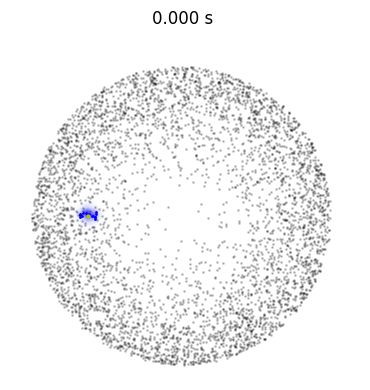
\includegraphics[width=0.49\textwidth]{simulation/4/frame_0.png}\hfill
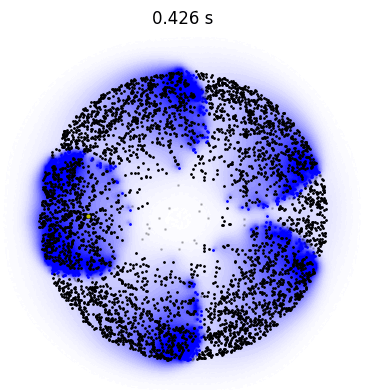
\includegraphics[width=0.49\textwidth]{simulation/4/frame_71.png}
\\[\smallskipamount]
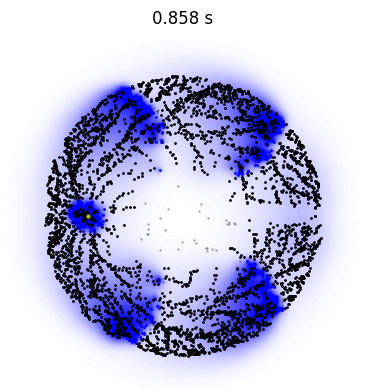
\includegraphics[width=0.49\textwidth]{simulation/4/frame_143.png}\hfill
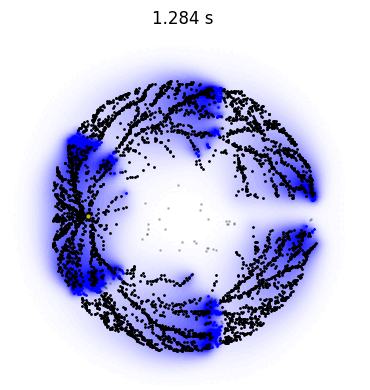
\includegraphics[width=0.49\textwidth]{simulation/4/frame_214.png}
\\[\smallskipamount]
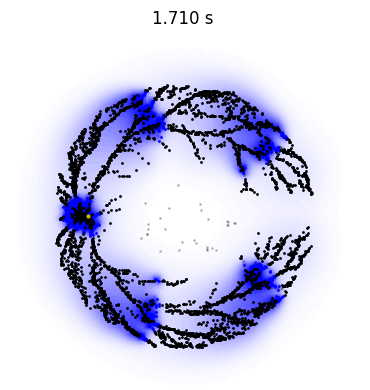
\includegraphics[width=0.49\textwidth]{simulation/4/frame_285.png}\hfill
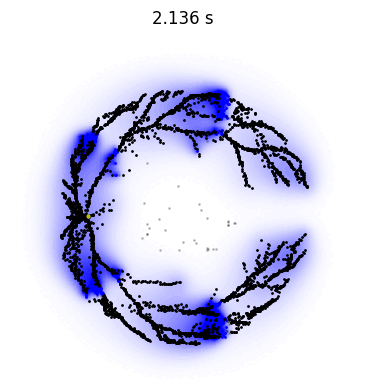
\includegraphics[width=0.49\textwidth]{simulation/4/frame_356.png}
\\[\smallskipamount]
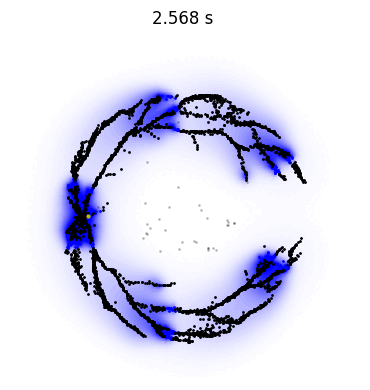
\includegraphics[width=0.49\textwidth]{simulation/4/frame_428.png}\hfill
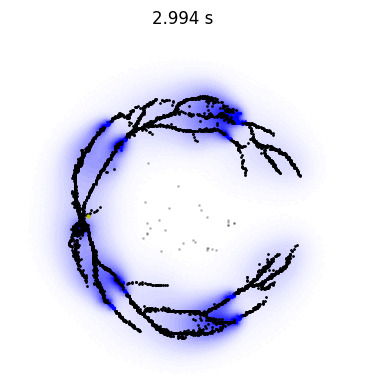
\includegraphics[width=0.49\textwidth]{simulation/4/frame_499.png}
\end{align*}
\end{minipage}
\begin{minipage}{0.45\textwidth}
\subsection{Even Lower Density Center}
To take the Low Density Center simulation to the extreme we further lowered the center density here.
Again we get a similar result to the Annulus simulation.
Compared to the Low Density Simulation a even more pronounced empty circle in the center emerges.
Because of the low density there are even a few particles (the grey ones) that never left their inactive state as they where never in reach of the chemical.
Note that the separation on the right is way more visible compared to the Low Density Center simulation.
\end{minipage}